% !TEX root = ../main.tex
% SECTION 5: FEDERN
% Inhalt: Liv Erne, Silvio Seiz — Form: ZSF-Template-Rework
% ============================================================

\StartChapter[ch:federn]{Federn}
\ZSFindex{Feder}

\begin{propertylist}[Funktionen von Federn]
\item Gewährleistung von Form- und Reibschluss
\item Speichern potentielle Energie
\item Ausgleich von Ausdehnung und Verschleiss
\item Dämpfung durch Reibung
\item Einstellen von Schwingverhalten
\end{propertylist}

\begin{figbox}[Kennlinien]
\centering
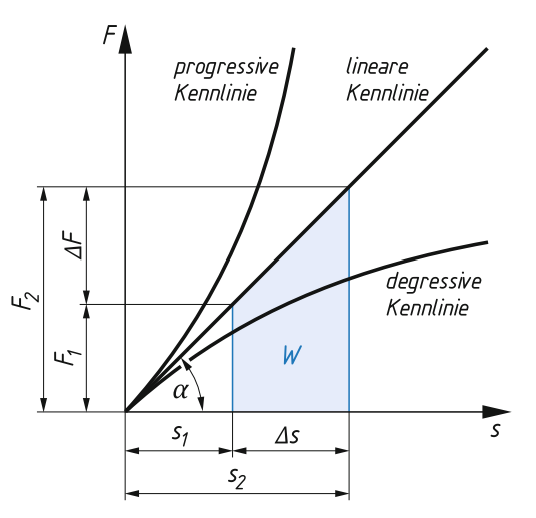
\includegraphics[width=0.5\linewidth,keepaspectratio]{graphics/schraubenfeder_kennlinie_linear_progressiv_degressiv.png}%
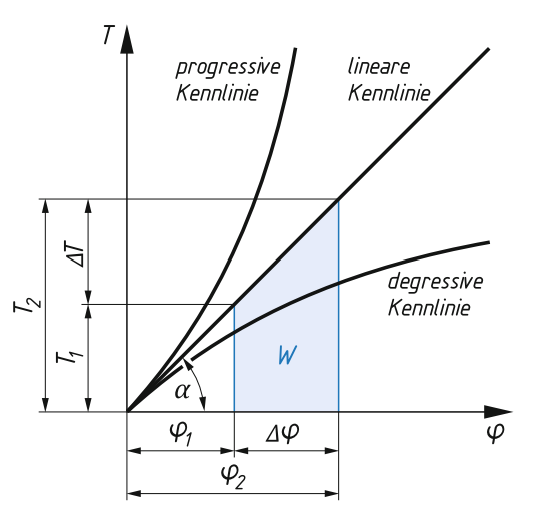
\includegraphics[width=0.5\linewidth,keepaspectratio]{graphics/drehfeder_kennlinie_linear_progressiv_degressiv.png}
\end{figbox}
\ZSFindex{Federkennlinie}

\begin{factlist}
\ZSFFact{Degressiv}{Feder wird mit steigender Belastung weicher.}
\ZSFFact{Progressiv}{Feder wird mit steigender Belastung härter.}
\end{factlist}
\ZSFgapS

\SubsectionBar{Federarbeit $\ZSFspringW$}
\ZSFindex{Federarbeit}

\begin{runintext}
Beim Spannen einer Feder wird Arbeit verrichtet, die die Feder beim Entspannen wieder abgibt. Jedoch entsteht durch die Reibung im angespannten Zustand Wärme (Dämpfungswert). Somit: $E_{Anspannen} > E_{Entspannen}$
\end{runintext}

\begin{formulabox}
\ZSFkeyword*{Federsysteme allgemein}:~$\ZSFspringW = \dfrac{1}{2}\cdot \ZSFspringF\cdot \ZSFspringS$
\formulanote{parallel: $\ZSFspringW = \dfrac{1}{2}\cdot \ZSFspringN\cdot \ZSFspringF\cdot \ZSFspringS$ mit $\ZSFspringN =$ Federn (mehrere Kräfte)}
\formulanote{in Reihe: $\ZSFspringW = \dfrac{1}{2}\cdot \ZSFspringF\cdot \ZSFspringN\cdot \ZSFspringS$ mit $\ZSFspringN =$ Federn (mehrere Wege)}
\end{formulabox}

\SubsectionBar[sec:zugdruckfedern]{Zug- und Druckfedern}
\ZSFindex{Zugfeder}
\ZSFindex{Druckfeder}

\begin{formulabox}
\ZSFkeyword*{Ersatz-Federrate $\ZSFspringRers$}: Parallelschaltung $\ZSFspringRers = \ZSFspringROne + \ZSFspringRTwo + \cdots + \ZSFspringRn$

Reihenschaltung $\ZSFspringRers = \dfrac{1}{\dfrac{1}{\ZSFspringROne} + \dfrac{1}{\ZSFspringRTwo} + \cdots + \dfrac{1}{\ZSFspringRn}}$

$\ZSFspringW = \dfrac{\ZSFspringR \cdot (\ZSFspringSTwo^2 - \ZSFspringSOne^2)}{2}\text{; } \ZSFspringWzus = \ZSFspringFv \cdot \ZSFspringDeltaS + \dfrac{1}{2}\, \ZSFspringR\, \ZSFspringDeltaS^2$
\formulanote{$\ZSFspringWzus$:~zusätzliche Federarbeit \ $\cdot$ \ $\ZSFspringFv$:~Vorspannkraft \ $\cdot$ \ $\ZSFspringDeltaS = \ZSFspringSTwo - \ZSFspringSOne$ \ $\cdot$ \ $\ZSFspringR$:~Federrate}
\formulanote{Kennlinie: je Abschnitt aktive Federn; Anschlag = aus; Steigung $\ZSFspringRers$.}
\end{formulabox}

\SubsubsectionBar{Schraubenfedern}
\ZSFindex{Schraubenfeder}

\begin{runintext}
\ZSFkeyword[Schraubenfeder]{Schraubenfedern} werden auf Torsion belastet.
\end{runintext}

\begin{figbox}[Schraubenfeder: Belastung und Geometrie]
\noindent
\begin{minipage}[c]{0.62\linewidth}
  \raggedright
  \begin{tikzpicture}[x=0.75pt,y=0.75pt,>=latex,font=\ZSFfontTableDense,every node/.style={scale=0.85}]
    % Seitenansicht: Axialkraft und Federweg
    \draw[densely dashed,gray] (30,7) -- (30,55);
    \draw[thick] (10,9) -- (50,9);
    \draw[thick] (10,51) -- (50,51);
    \draw[densely dashed,gray] (10,57) -- (50,57);
    \draw[very thick,\chaptercolor,smooth,domain=0:1440,samples=100]
      plot ({30+15*sin(\x)},{13+\x/41.15});
    \draw[->,thick,\chaptercolor] (30,63) -- (30,53) node[pos=0,left] {$\ZSFspringF$};
    \draw[->,thick,\chaptercolor] (30,-1) -- (30,7) node[pos=0,left] {$\ZSFspringF$};
    \draw[<->,thin] (6,51) -- (6,57) node[midway,left] {$\ZSFspringS$};

    % Draufsicht: Aussen-, Innen-, mittlerer und Drahtdurchmesser
    \draw[very thick,\chaptercolor] (100,29) circle (20);
    \draw[very thick,\chaptercolor] (100,29) circle (12);
    \draw[densely dashed,gray] (100,29) circle (16);
    \draw[thin] (80,49) -- (80,55);
    \draw[thin] (120,49) -- (120,55);
    \draw[<->,thin] (80,53) -- (120,53) node[midway,fill=white,inner sep=0.5pt] {$\ZSFspringDe$};
    \draw[thin] (88,9) -- (88,3);
    \draw[thin] (112,9) -- (112,3);
    \draw[<->,thin] (88,5) -- (112,5) node[midway,fill=white,inner sep=0.5pt] {$\ZSFspringDi$};
    \draw[<->,thin] (84,29) -- (116,29) node[midway,fill=white,inner sep=0.5pt] {$\ZSFspringDbig$};
    \draw[<->,thin] (100,41) -- (100,49) node[midway,right] {$\ZSFspringD$};
  \end{tikzpicture}
\end{minipage}%
\hfill
\begin{minipage}[c]{0.34\linewidth}
  \centering
  \ZSFReadableOn
  \ZSFkeyword*{Federrate}:~$\ZSFspringF = \ZSFspringR \cdot \ZSFspringS$
  \ZSFgapL
  $\displaystyle \ZSFspringDbig = \ZSFspringDi + \ZSFspringD = \ZSFspringDe -\ZSFspringD$
\end{minipage}%
\par
\ZSFgapS
\hrule
\ZSFgapS
\ZSFReadableOn
{\centering $\displaystyle \ZSFspringR = \dfrac{\ZSFspringG \cdot \ZSFspringD^4}{8 \cdot \ZSFspringDbig^3 \cdot \ZSFspringNCoils} \qquad \ZSFspringF = \dfrac{\ZSFspringG \cdot \ZSFspringD^4 \cdot \ZSFspringS}{8 \cdot \ZSFspringDbig^3 \cdot \ZSFspringNCoils}$ \par}
\ZSFgapS
{\centering $\displaystyle \ZSFspringTauT = \dfrac{\ZSFspringMt}{\ZSFspringWt} = \dfrac{16 \cdot \ZSFspringMt}{\pi \cdot \ZSFspringD^3} = \ZSFspringG \cdot \tan\ZSFspringGamma \approx \ZSFspringG \cdot \ZSFspringGamma \qquad \ZSFspringMt = \dfrac{\ZSFspringF\cdot \ZSFspringDbig}{2}$ \par}
\formulanote{$\ZSFspringG$:~Schubmodul \ $\cdot$ \ $\ZSFspringNCoils$:~aktive Windungszahl \ $\cdot$ \ $\ZSFspringGamma$:~Schubwinkel}
\end{figbox}
\ZSFindex{Federrate}

\begin{propertylist}[Gabelfedern]
\item Kleine Unebenheit $\rightarrow$ kleine Federung
\item Grosse Unebenheit $\rightarrow$ grosse Federung
\end{propertylist}
\ZSFindex{Gabelfeder}

\SubsubsectionBarOnNewColumn{Tellerfedern}
\ZSFindex{Tellerfeder}

\begin{runintext}
Halten sehr hohe Druckkräfte aus. Sie werden jedoch nie auf Block belastet ($\ZSFspringAlpha$ = 0°), weil man sonst im Bereich der plastischen Verformung ist. \ZSFdanger{Regel: $\ZSFspringS \leq 0,75 \cdot \ZSFspringHZero$}
\end{runintext}

\ZSFfig[0.65]{graphics/tellerfeder_kennwerte_abmessungen.png}{}{}
%\ZSFfig{graphics/tellerfedern_kennlinien.png}{Tellerfedern Kennlinien}{}

\begin{propertylist}[Kennlinien]
\ZSFFact{Linear}{$\ZSFspringHZero/\ZSFspringT\approx 0,4$}
\ZSFFact{Degressiv}{$\ZSFspringHZero/\ZSFspringT \approx 0,75$}
\ZSFFact{Stark degressiv (Plateau)}{$\ZSFspringHZero/\ZSFspringT \approx 1,4 \rightarrow$ Mit der Zeit verschwindet das Plateau durch Abnutzung, meistens bei Dauerbetrieb.}
\ZSFFact{Kraftmaximum erreicht}{$\ZSFspringHZero/\ZSFspringT \geq 1,4$}
\end{propertylist}

\SubsubsectionBar{Federpaket und Federsäule}
\ZSFindex{Federpaket}
\ZSFindex[federsaule]{Federsäule}

%
\ZSFfig[1.0]{graphics/tellerfeder_paket_saeule_kennlinie.pdf}{}{}

\begin{tablebox}[Paket ($\ZSFspringN$ parallel) vs. Säule ($\ZSFspringI$ in Reihe)]
\begin{ZSFtable}{Y{1.0} Y{1.0} Y{1.0}}
\ZSFheaderRow \ZSFhead{gegenüber 1 Teller} & \ZSFhead{Paket (parallel)} & \ZSFhead{Säule (Reihe)} \\
Aufbau & \ZSFtablestrut $\ZSFspringN$ Teller parallel & $\ZSFspringI$ Teller in Reihe \\
Federrate & \ZSFtablestrut $\ZSFspringRers=\ZSFspringN\cdot \ZSFspringR$ (härter) & $\ZSFspringRers=\dfrac{\ZSFspringR}{\ZSFspringI}$ (weicher) \\
bei gleichem $\ZSFspringS$:~Kraft & \ZSFtablestrut $\ZSFspringN$-fach: $\ZSFspringF\cdot \ZSFspringN$ & $\ZSFspringI$-tel: $\ZSFspringF/\ZSFspringI$ \\
bei gleichem $\ZSFspringF$:~Weg & \ZSFtablestrut $\ZSFspringN$-tel: $\ZSFspringS/\ZSFspringN$ & $\ZSFspringI$-fach: $\ZSFspringS\cdot \ZSFspringI$
\end{ZSFtable}
\formulanote{Paket teilt die Last (jeder Teller trägt $\ZSFspringF/\ZSFspringN$), Säule teilt den Weg. Gleiche Pakete ($\ZSFspringN$ parallel, $\ZSFspringI$ in Reihe): $\ZSFspringRers=\dfrac{\ZSFspringN}{\ZSFspringI}\cdot \ZSFspringR$}
\formulanote{Ungleiche Pakete in Reihe ($m$ Pakete mit $\ZSFspringN_k$ Teller): $\ZSFspringRers = \dfrac{\ZSFspringR}{\sum_{k=1}^m \frac{1}{\ZSFspringN_k}}$ \ $\cdot$ \ \ZSFdanger{Schwächstes Paket schlägt zuerst an} $\rightarrow$ Knick-Kennlinie}
\end{tablebox}

\SubsectionBar[sec:drehfedern]{Drehfedern}
\ZSFindex{Drehfeder}
\ZSFindex{Schenkelfeder}

\begin{figbox}[Schenkelfedern]
\centering
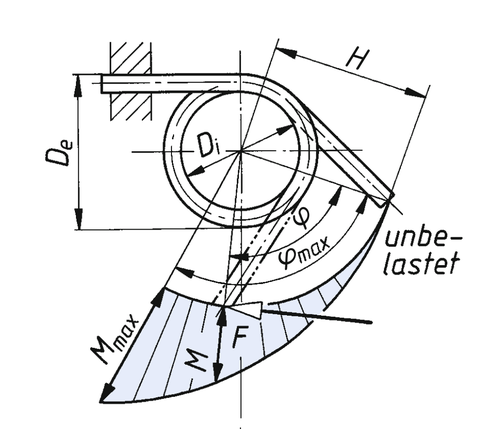
\includegraphics[width=0.4\linewidth,keepaspectratio]{graphics/drehfeder_kennwerte_moment_winkel.png}%
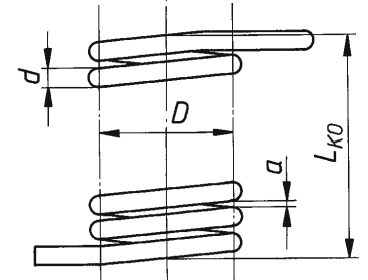
\includegraphics[width=0.35\linewidth,keepaspectratio]{graphics/drehfeder_abmessungen_drahtdurchmesser_federdurchmesser_lk0.png}
\end{figbox}

\begin{formulabox}
$\ZSFspringM = \ZSFspringR \cdot \ZSFspringPhi$

$\ZSFspringR = \dfrac{\pi}{180°}\cdot \dfrac{\ZSFspringE \cdot \ZSFspringD^4}{64 \cdot \ZSFspringDbig\cdot \ZSFspringNCoils}$
\formulanote{mit Normalkraft im Material $\ZSFspringE$}
$\ZSFspringW = \dfrac{\ZSFspringR \cdot (\ZSFspringPhiTwo^2 - \ZSFspringPhiOne^2)}{2} \text{, falls } \ZSFspringPhiOne = 0\text{; } \ZSFspringW = \dfrac{\ZSFspringMTwo \cdot \ZSFspringPhiTwo}{2}$
\end{formulabox}

\SubsubsectionBar{Drehstabfedern}
\ZSFindex{Drehstabfeder}

\begin{splitbox}[0.6]
\centering
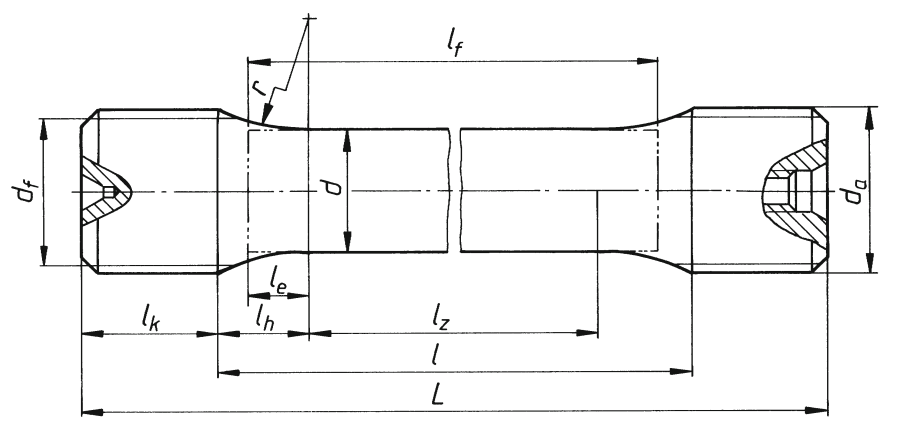
\includegraphics[width=\linewidth,keepaspectratio]{graphics/drehstabfeder_kennwerte_abmessungen.png}
\tcblower
{\centering $\displaystyle \ZSFspringR = \dfrac{\pi}{180°}\cdot \dfrac{\pi \cdot \ZSFspringG \cdot  \ZSFspringD^4}{32 \cdot \ZSFspringLf}$\par}
\ZSFgapXS
\formulanote{mit Torsion im Material $\ZSFspringG$}
\end{splitbox}

\SubsectionBarOnNewColumn[sec:biegefedern]{Biegefedern}
\ZSFindex{Biegefeder}
\ZSFindex{Blattfeder}

\ZSFfig[1.0]{graphics/v7_blattfeder_q1_werte.png}{}{}

\begin{formulabox}
$\ZSFspringR = \dfrac{\ZSFspringB \cdot \ZSFspringH^3 \cdot  \ZSFspringE}{\ZSFspringQOne \cdot \ZSFspringL^3}$
\end{formulabox}

\SubsubsectionBar{Zweiarmige Blattfedern}

\begin{splitbox}[0.45]
\centering
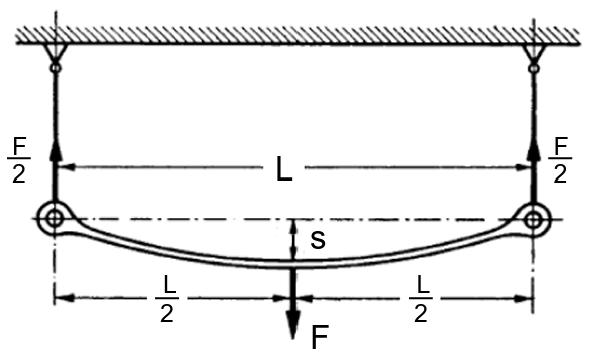
\includegraphics[width=\linewidth,keepaspectratio]{graphics/v7_zweiarmige_blattfeder_kennwerte.png}
\tcblower
$\approx$ Parallelschaltung von zwei einarmigen Blattfedern.

$\ZSFspringRers = \ZSFspringROne + \ZSFspringRTwo = 2\cdot \ZSFspringR$
\end{splitbox}

\begin{runintext}
Anwendung geschichteter Blattfedern: Federung von schweren Fahrzeugen wie Güterwagons, da zwischen den Federn starke Reibung auftritt, die dämpfend wirkt.
\end{runintext}

\SubsubsectionBar{Schnappverbindungen}
\ZSFindex{Schnappverbindung}

\begin{runintext}
Zwei einarmige Blattfedern mit Schnapphaken, die in einer Rastvorrichtung einschnappen können.
\end{runintext}

\ZSFfig[0.75]{graphics/v7_schnappverbindung_kennwerte.png}{}{}

\begin{factlist}
\item $\ZSFspringAlphaTwo < 90$° ist lösbar
\item $\ZSFspringAlphaTwo \geq 90$° nur mit einem Lösemechanismus lösbar
\end{factlist}

\begin{formulabox}
$\ZSFspringF = \ZSFspringR \cdot \ZSFspringS \qquad \ZSFspringR = \dfrac{\ZSFspringB \cdot \ZSFspringH^3 \cdot  \ZSFspringE}{4 \cdot \ZSFspringL^3}$
\end{formulabox}
